\chapter{Rig Construction}\label{sc:rig}
Based on the system requirements specified in \cref{sec:requirements} and the hardware components presented in \cref{chp:tech}, there have been construct two setup design ideas for constructing a rig, which will comply to the requirements and use the selected hardware components.

Both setup design ideas are designed to track a object in a 3D space for this two things components are used, firstly a laser pointer to mark the target and secondly the component for moving the laser point in a 3D space, this component is the DC motor which are include in the \acrfull{nxt} set. It has been selected to use one motor for horizontal movement and one for vertical movement.


To use the \gls{nxt} motors for moving a pointer, a rig is constructed with Lego bricks. This section presents two ideas to construct the rig and decides upon the presented setups. When evaluating the two setups it is important to assess the impact on factors such as stability of the rig, rotational freedom and the centres of the horizontal and vertical rotation axes.

\section{First Setup}\label{sec:first_setup}
The first setup, as seen on \cref{fig:rig_flat}, has a gear directly on a motor used for rotation of the vertical axis, illustrated on \cref{fig:rotation_defs}. The gear connected to the motor has a 90\degree\ connection to another gear which is part of a rotational turret, a close-up of this is shown on \cref{fig:rig_horizontal_base}. The other motor for rotation of the horizontal axis is fixated on the rotational turret. The motor has multiple fix points which is greatly beneficial for the stability.

A complication that arise from the setup is the need to define an offset, as the origin of the global coordinate system has its base in the intersection of the two axes. The offset is the distance between the base point to the vertical axis, which is the motor that has the laser attached to it. The offset is used when a rotation in the vertical plane is performed as the base point for the horizontal axis rotation is moved in the global coordinate system, and a calculation of the new position must be executed. Regarding the rotational freedom, the vertical rotation motor can move freely, when not considering the other motor. Restrictions for the rotations are that a cable must be connected to the motor for the horizontal rotation, which restricts the otherwise freely moving vertical motor. Furthermore the pointing device that must be connected to the horizontal motor, restricting the pointer in being able to do a 360\degree\ rotation. A close-up of the setup for the pointer is seen on \cref{fig:rig_horizontal_rotation}.
\begin{figure}[H]
	\begin{minipage}{0.5\textwidth}
		\centering
    	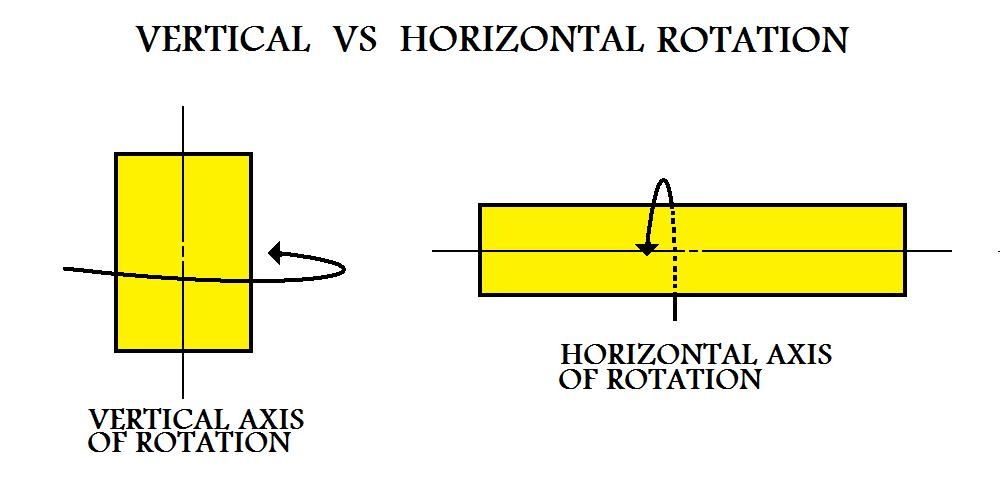
\includegraphics[width=0.80\textwidth]{graphics/rotation_definitions.jpg}
    	\caption{Illustrations of rotational axes \cite{rotation_definitions}}
    	\label{fig:rotation_defs}
	\end{minipage}
	\begin{minipage}{0.5\textwidth}
		\centering
    	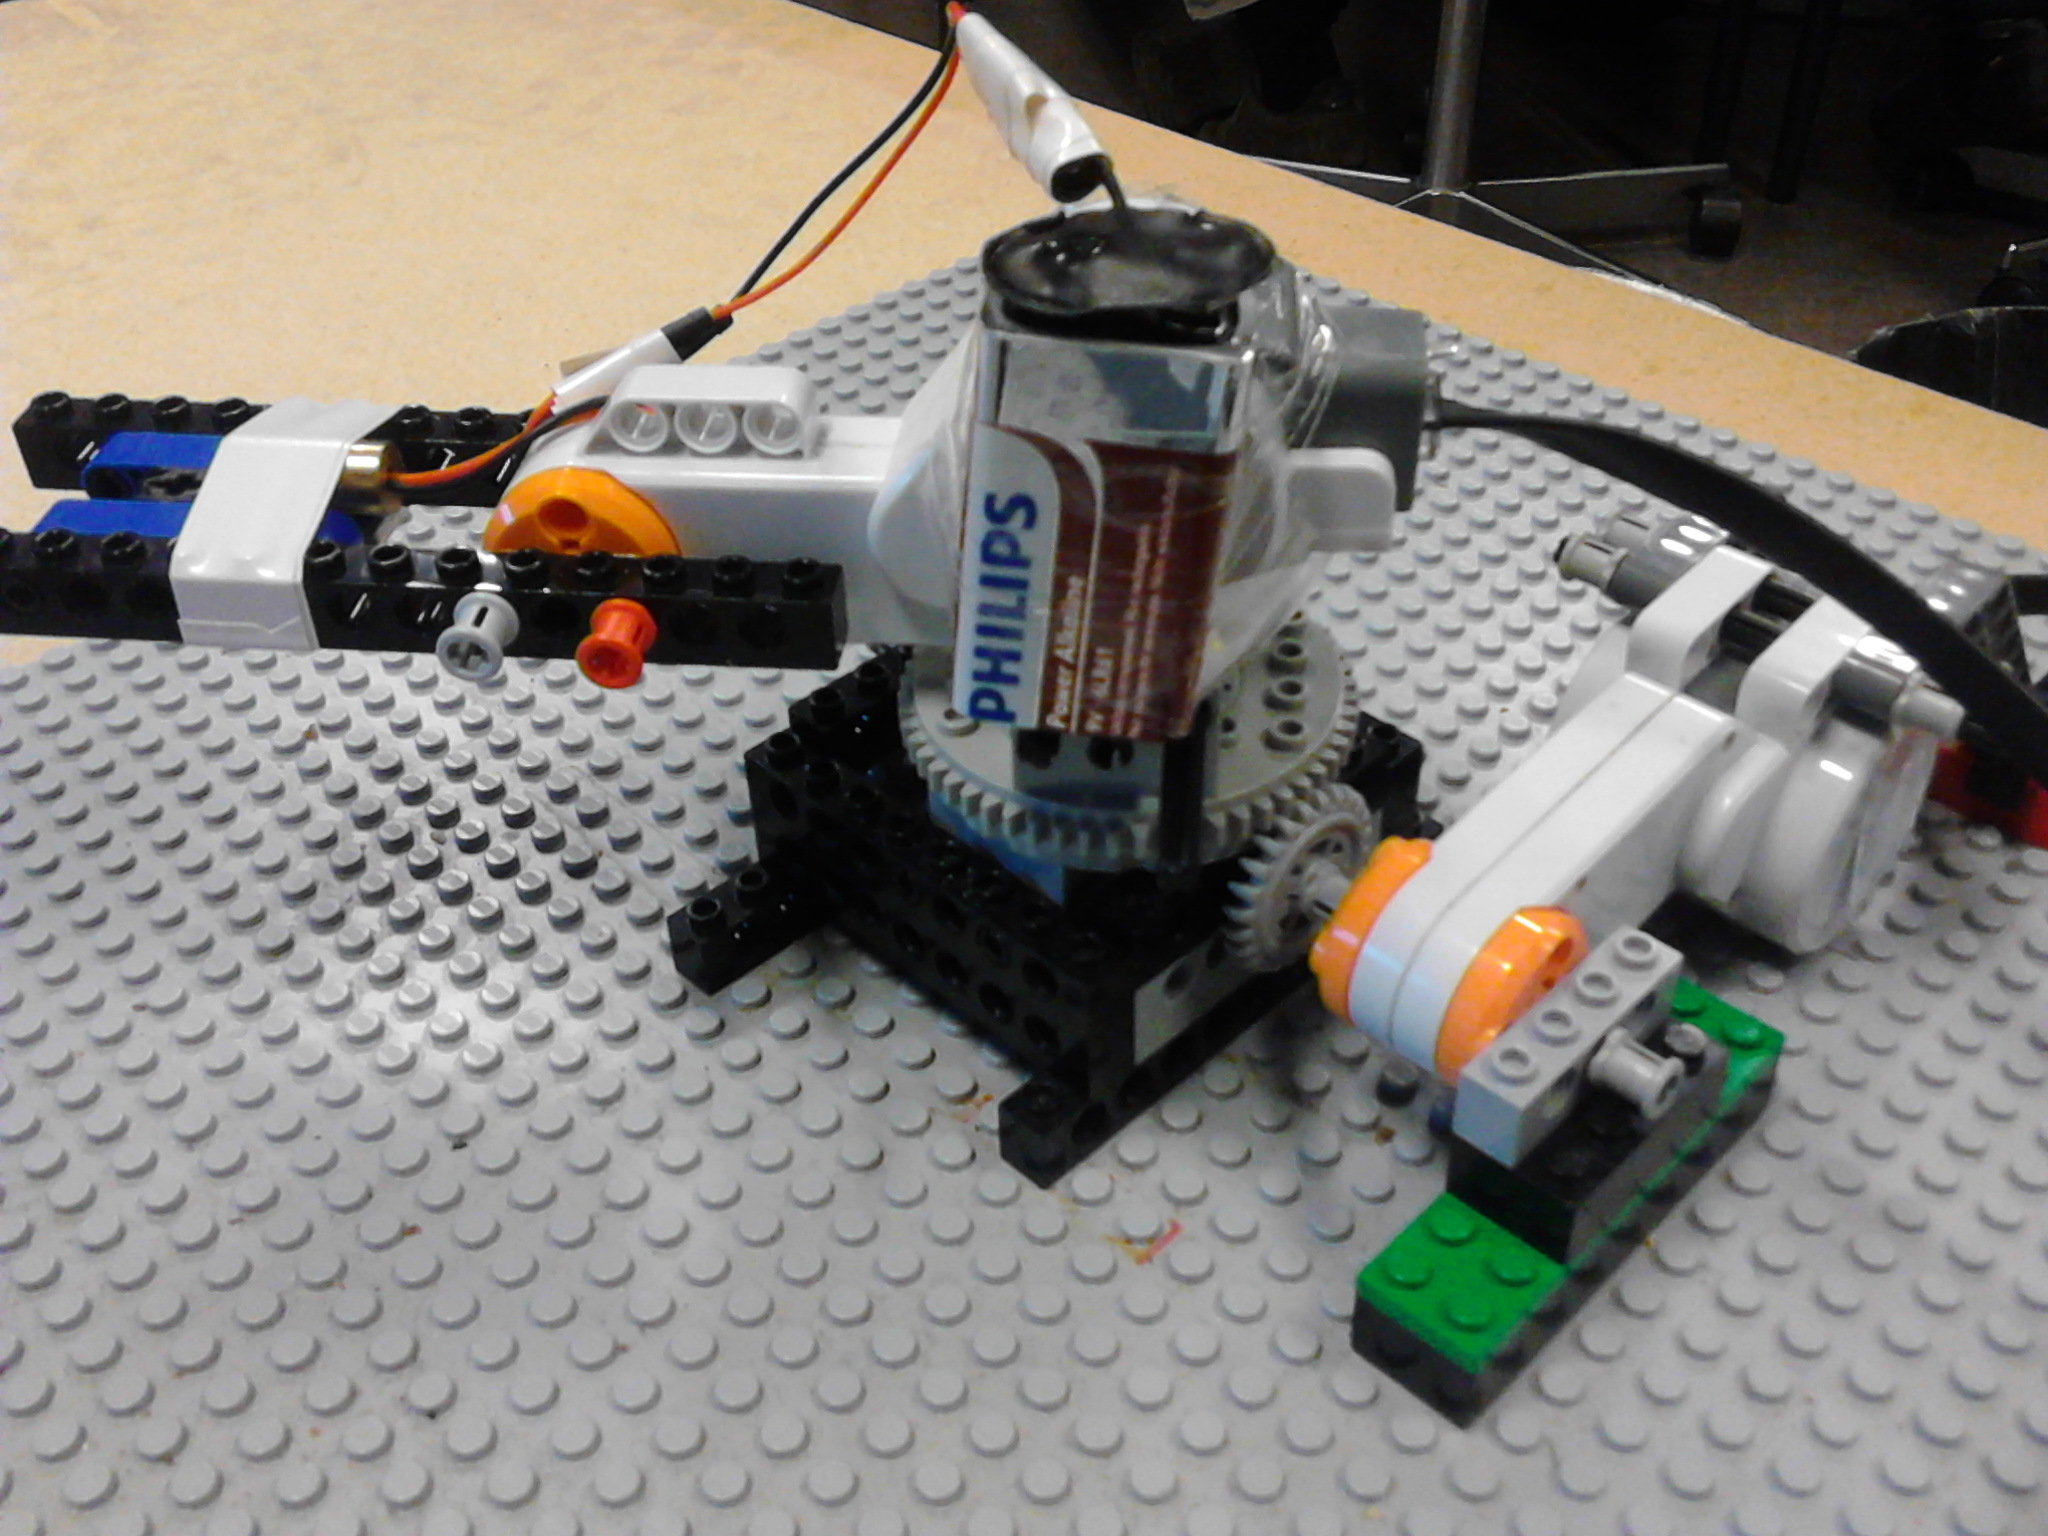
\includegraphics[width=0.80\textwidth]{graphics/rig/rig_flat_entire.jpg}
    	\caption{First setup}
	    \label{fig:rig_flat}
	\end{minipage}
\end{figure}

\begin{figure}[H]
    \begin{minipage}{0.5\textwidth}
    	\centering
    	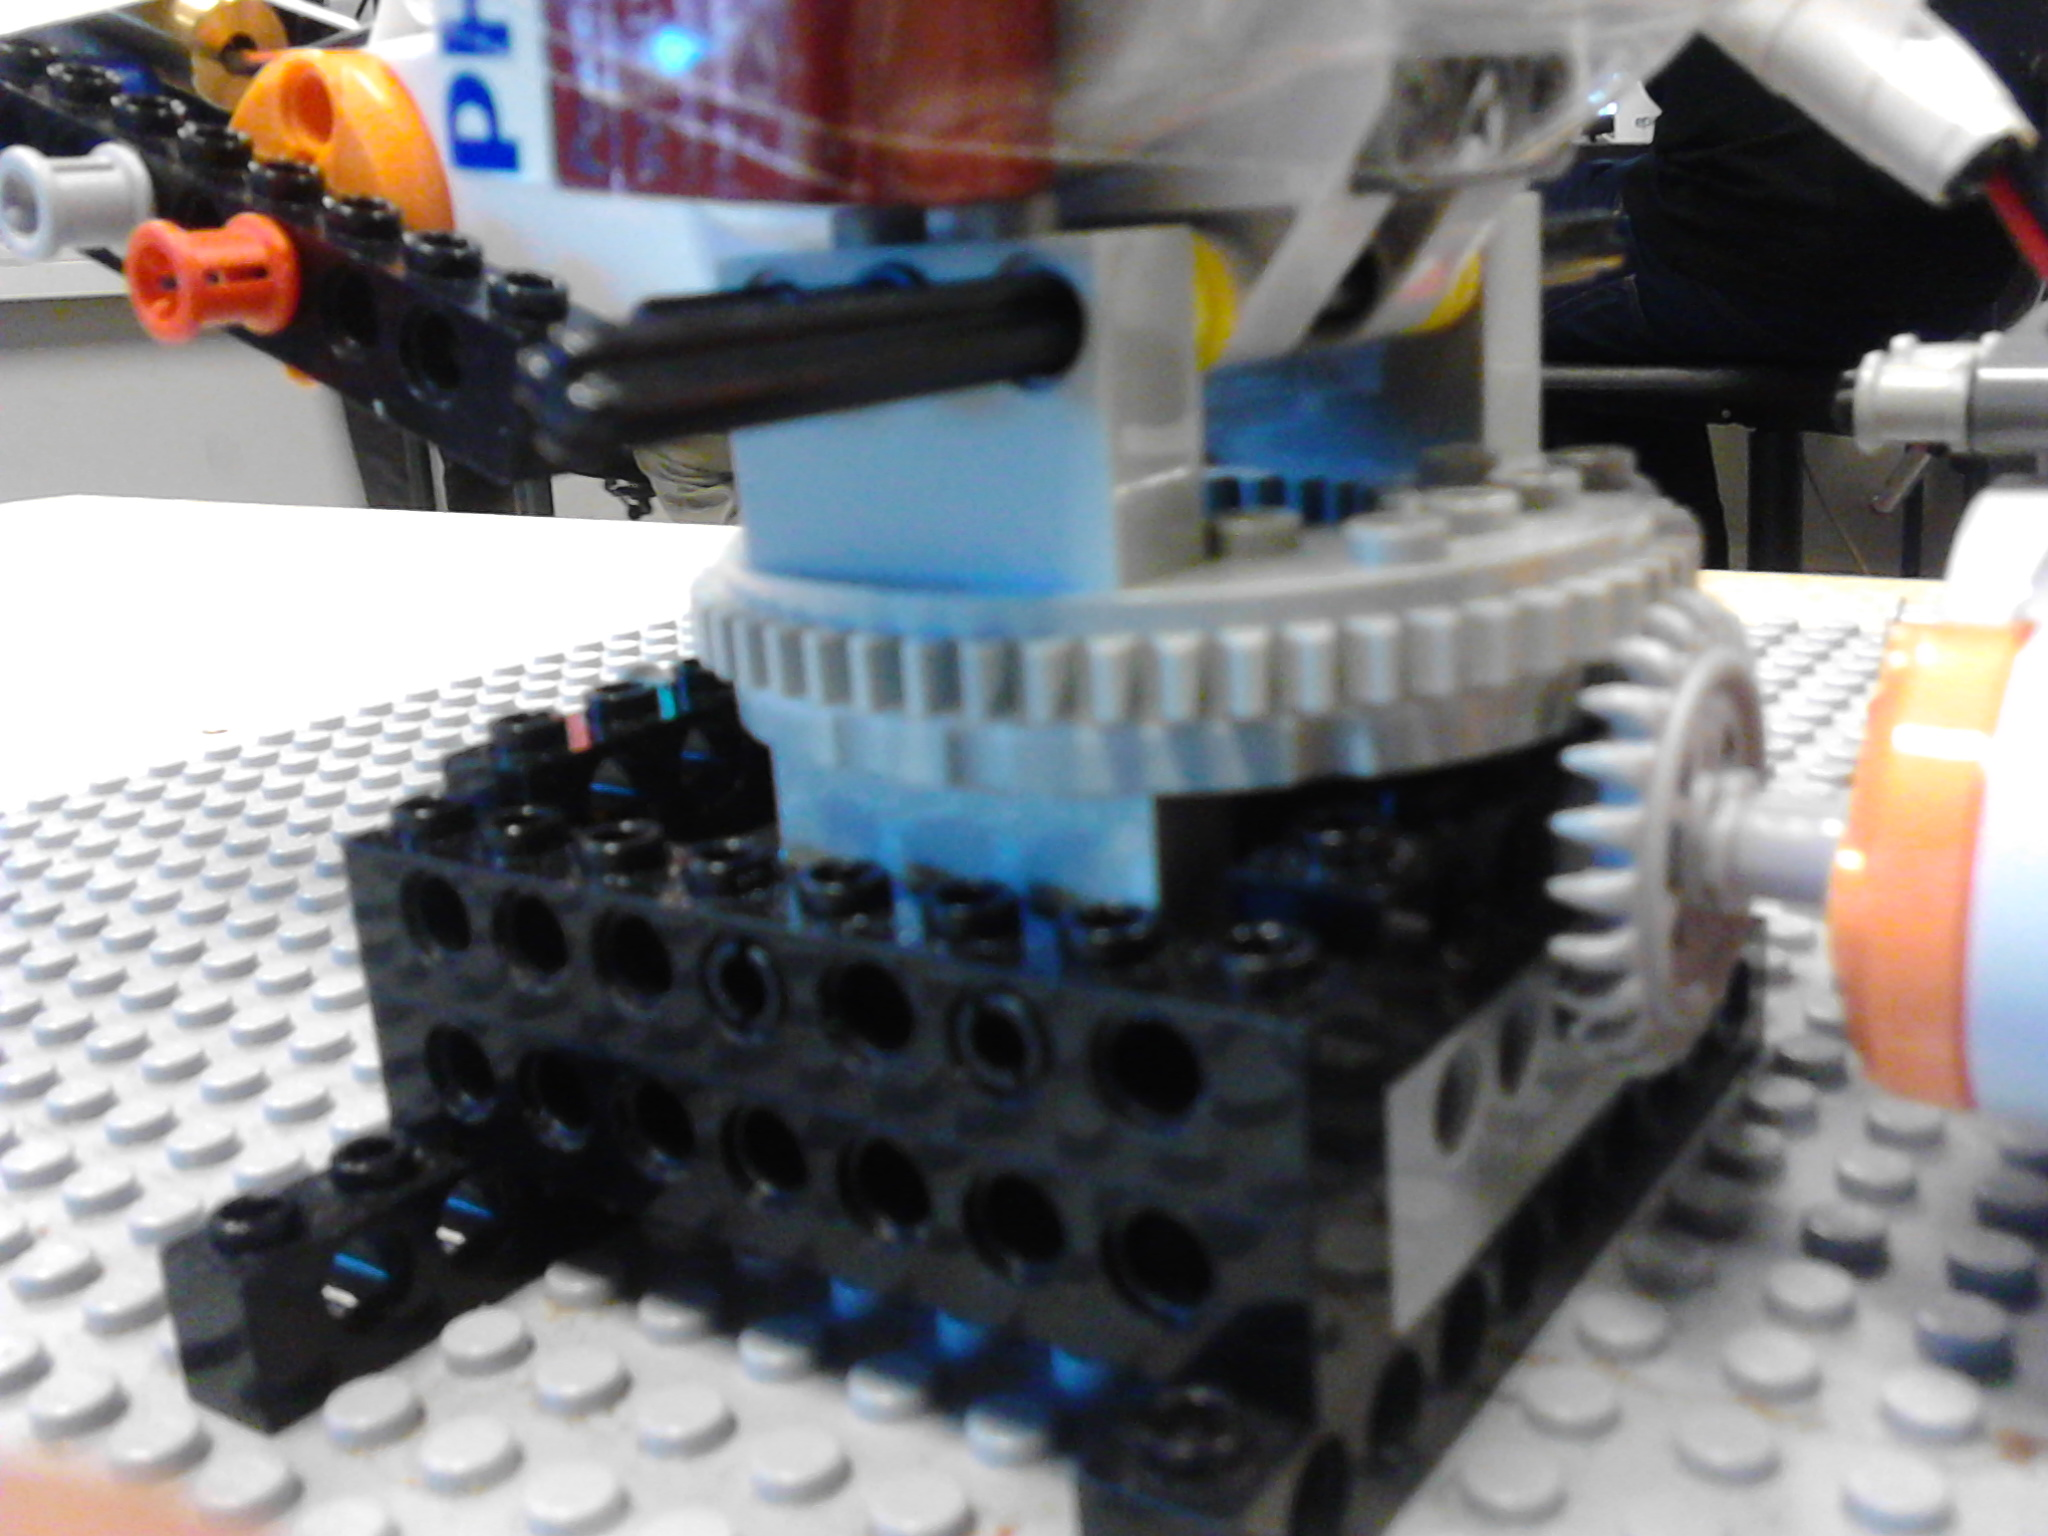
\includegraphics[width=0.80\textwidth]{graphics/rig/rig_horizontal_turret.jpg}
    	\caption{close-up of rotational turret for first setup}
    	\label{fig:rig_horizontal_base}
    \end{minipage}%
	\begin{minipage}{0.5\textwidth}
    	\centering
    	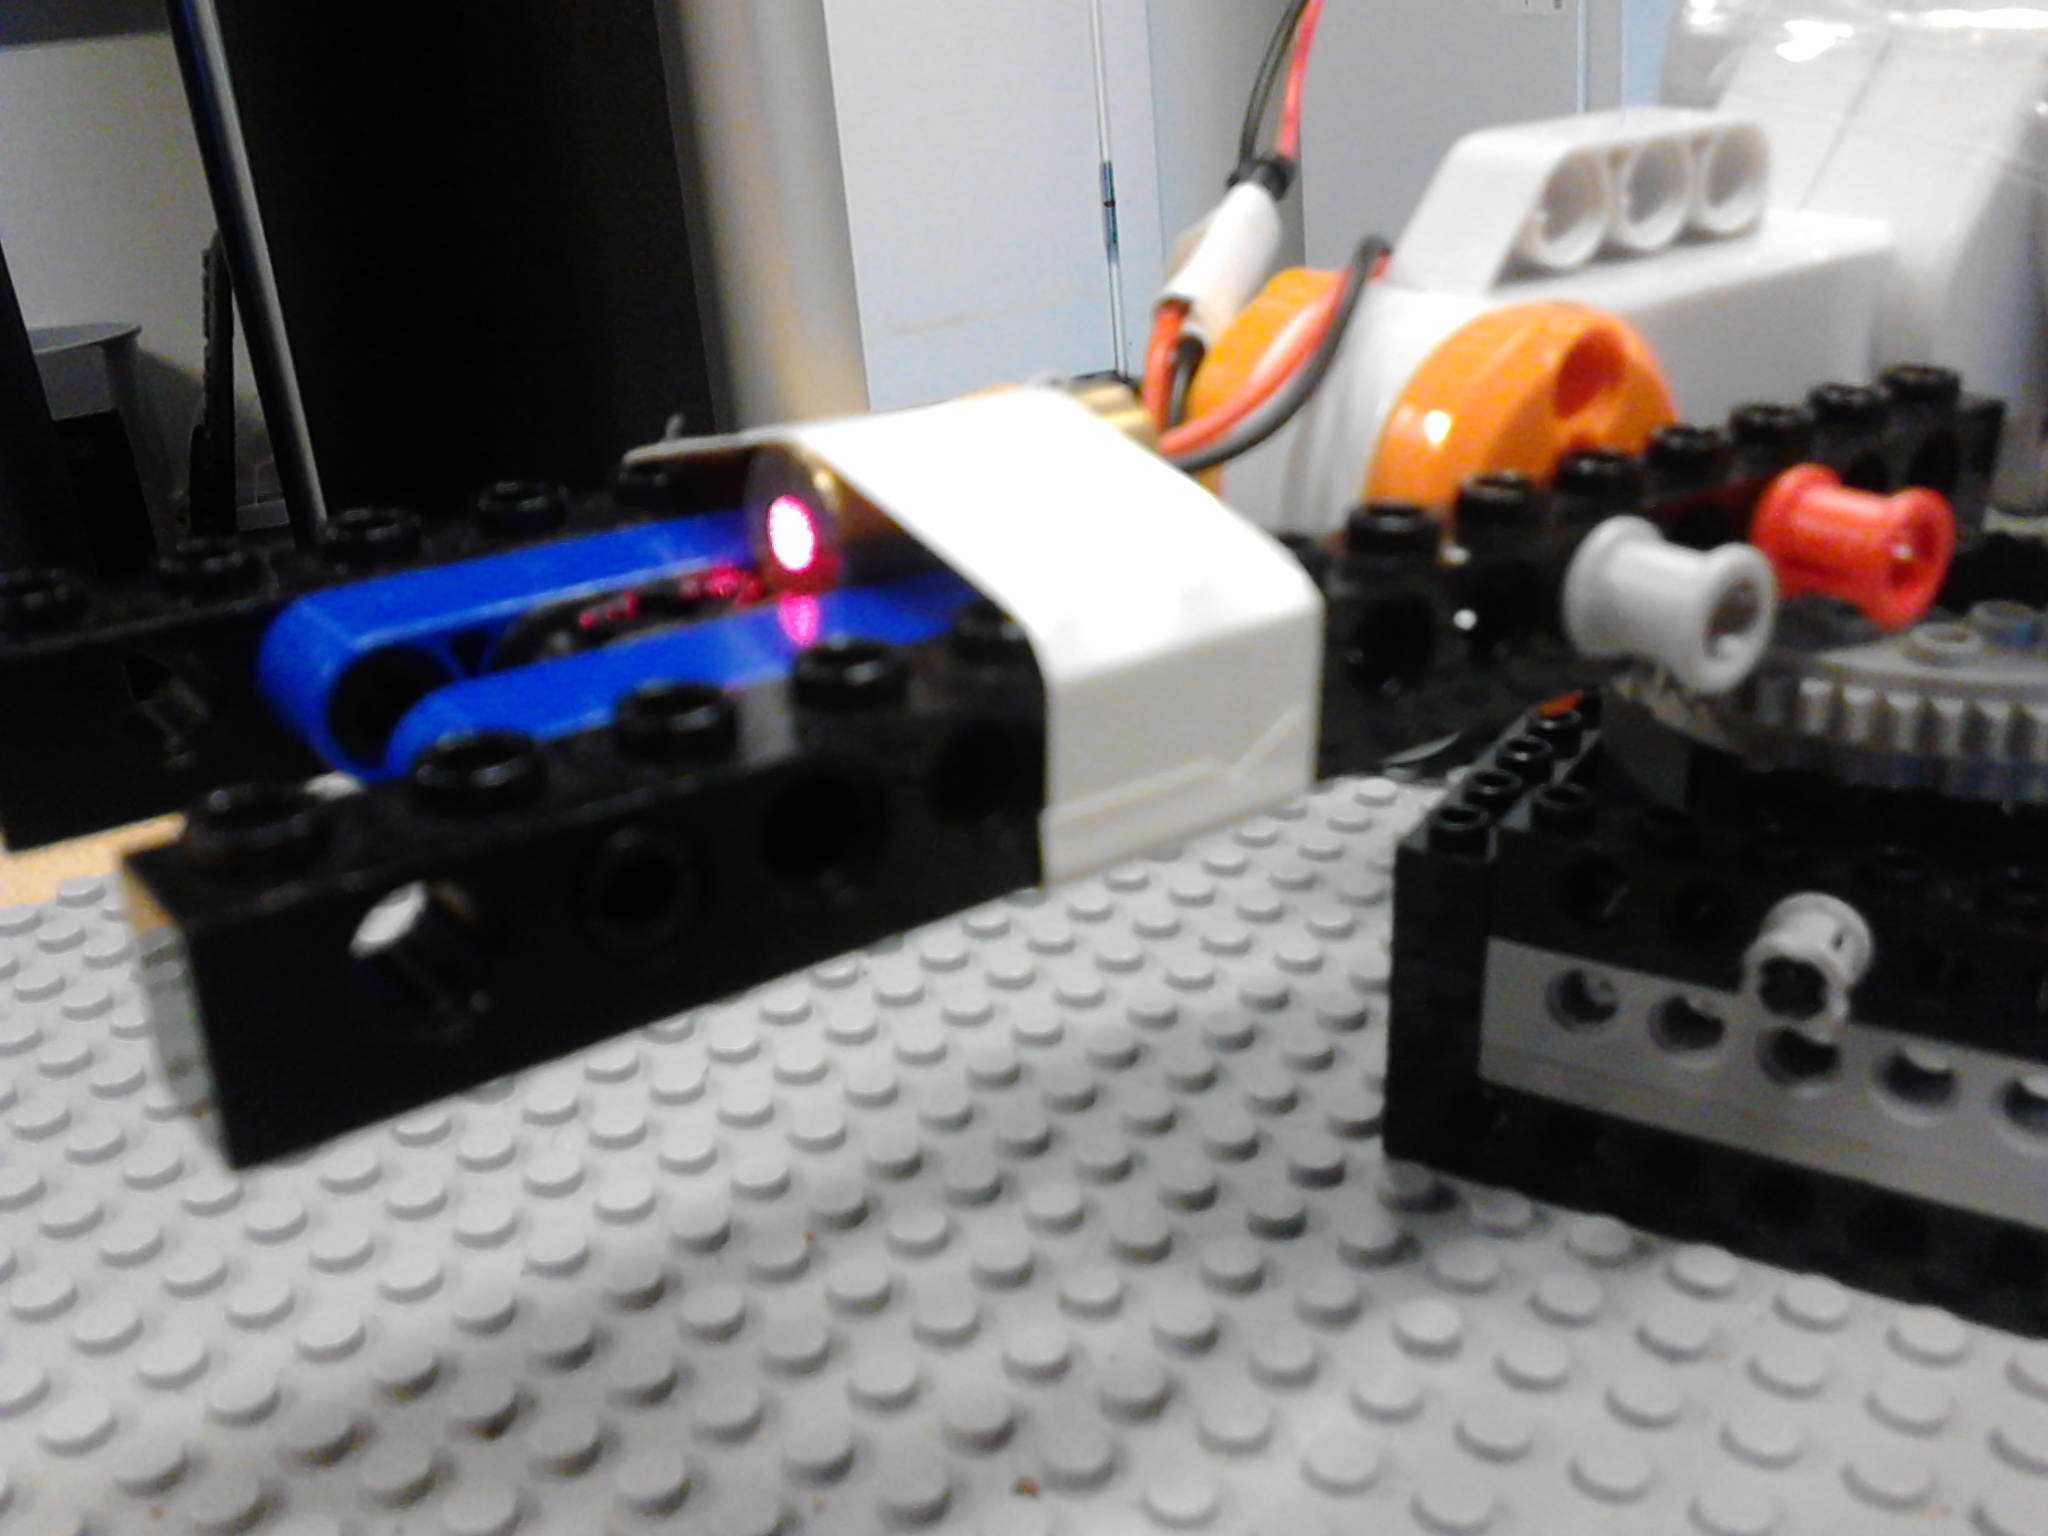
\includegraphics[width=0.80\textwidth]{graphics/rig/rig_vertical.jpg}
    	\caption{close-up of setup for rotation of horizontal axis}
    	\label{fig:rig_horizontal_rotation}
	\end{minipage}
\end{figure}

\section{Second Setup}
The second setup utilizes the same base structure for the rotation of the vertical axes with the 90\degree\ connected gears. But the Lego turret brick is of another model which results in the motor for horizontal rotation to be placed upright. A gain from this setup is that the rotational bases are placed directly on top of each other making the definitions thereof more simple than the first setup, as the base point of the horizontal rotational axis does not require recalculation. However, the upright placement of the motor results in fewer fix points and a more unstable connection, having the pointer vibrate greatly when either motor is moved. Another version of the setup gave better stability but resulted in the upright motor base point to be pushed off-centre. Pictures of both versions are shown in \cref{fig:rig_unstable} and \cref{fig:rig_stable}. Lastly the rotational freedom for the second setup is the same as for the first setup where the pointer is connected to the horizontal rotation axis, and a cable is connected to the motor, which restricts the rotation of the vertical rotational axis.

\begin{figure}[H]
    \centering
    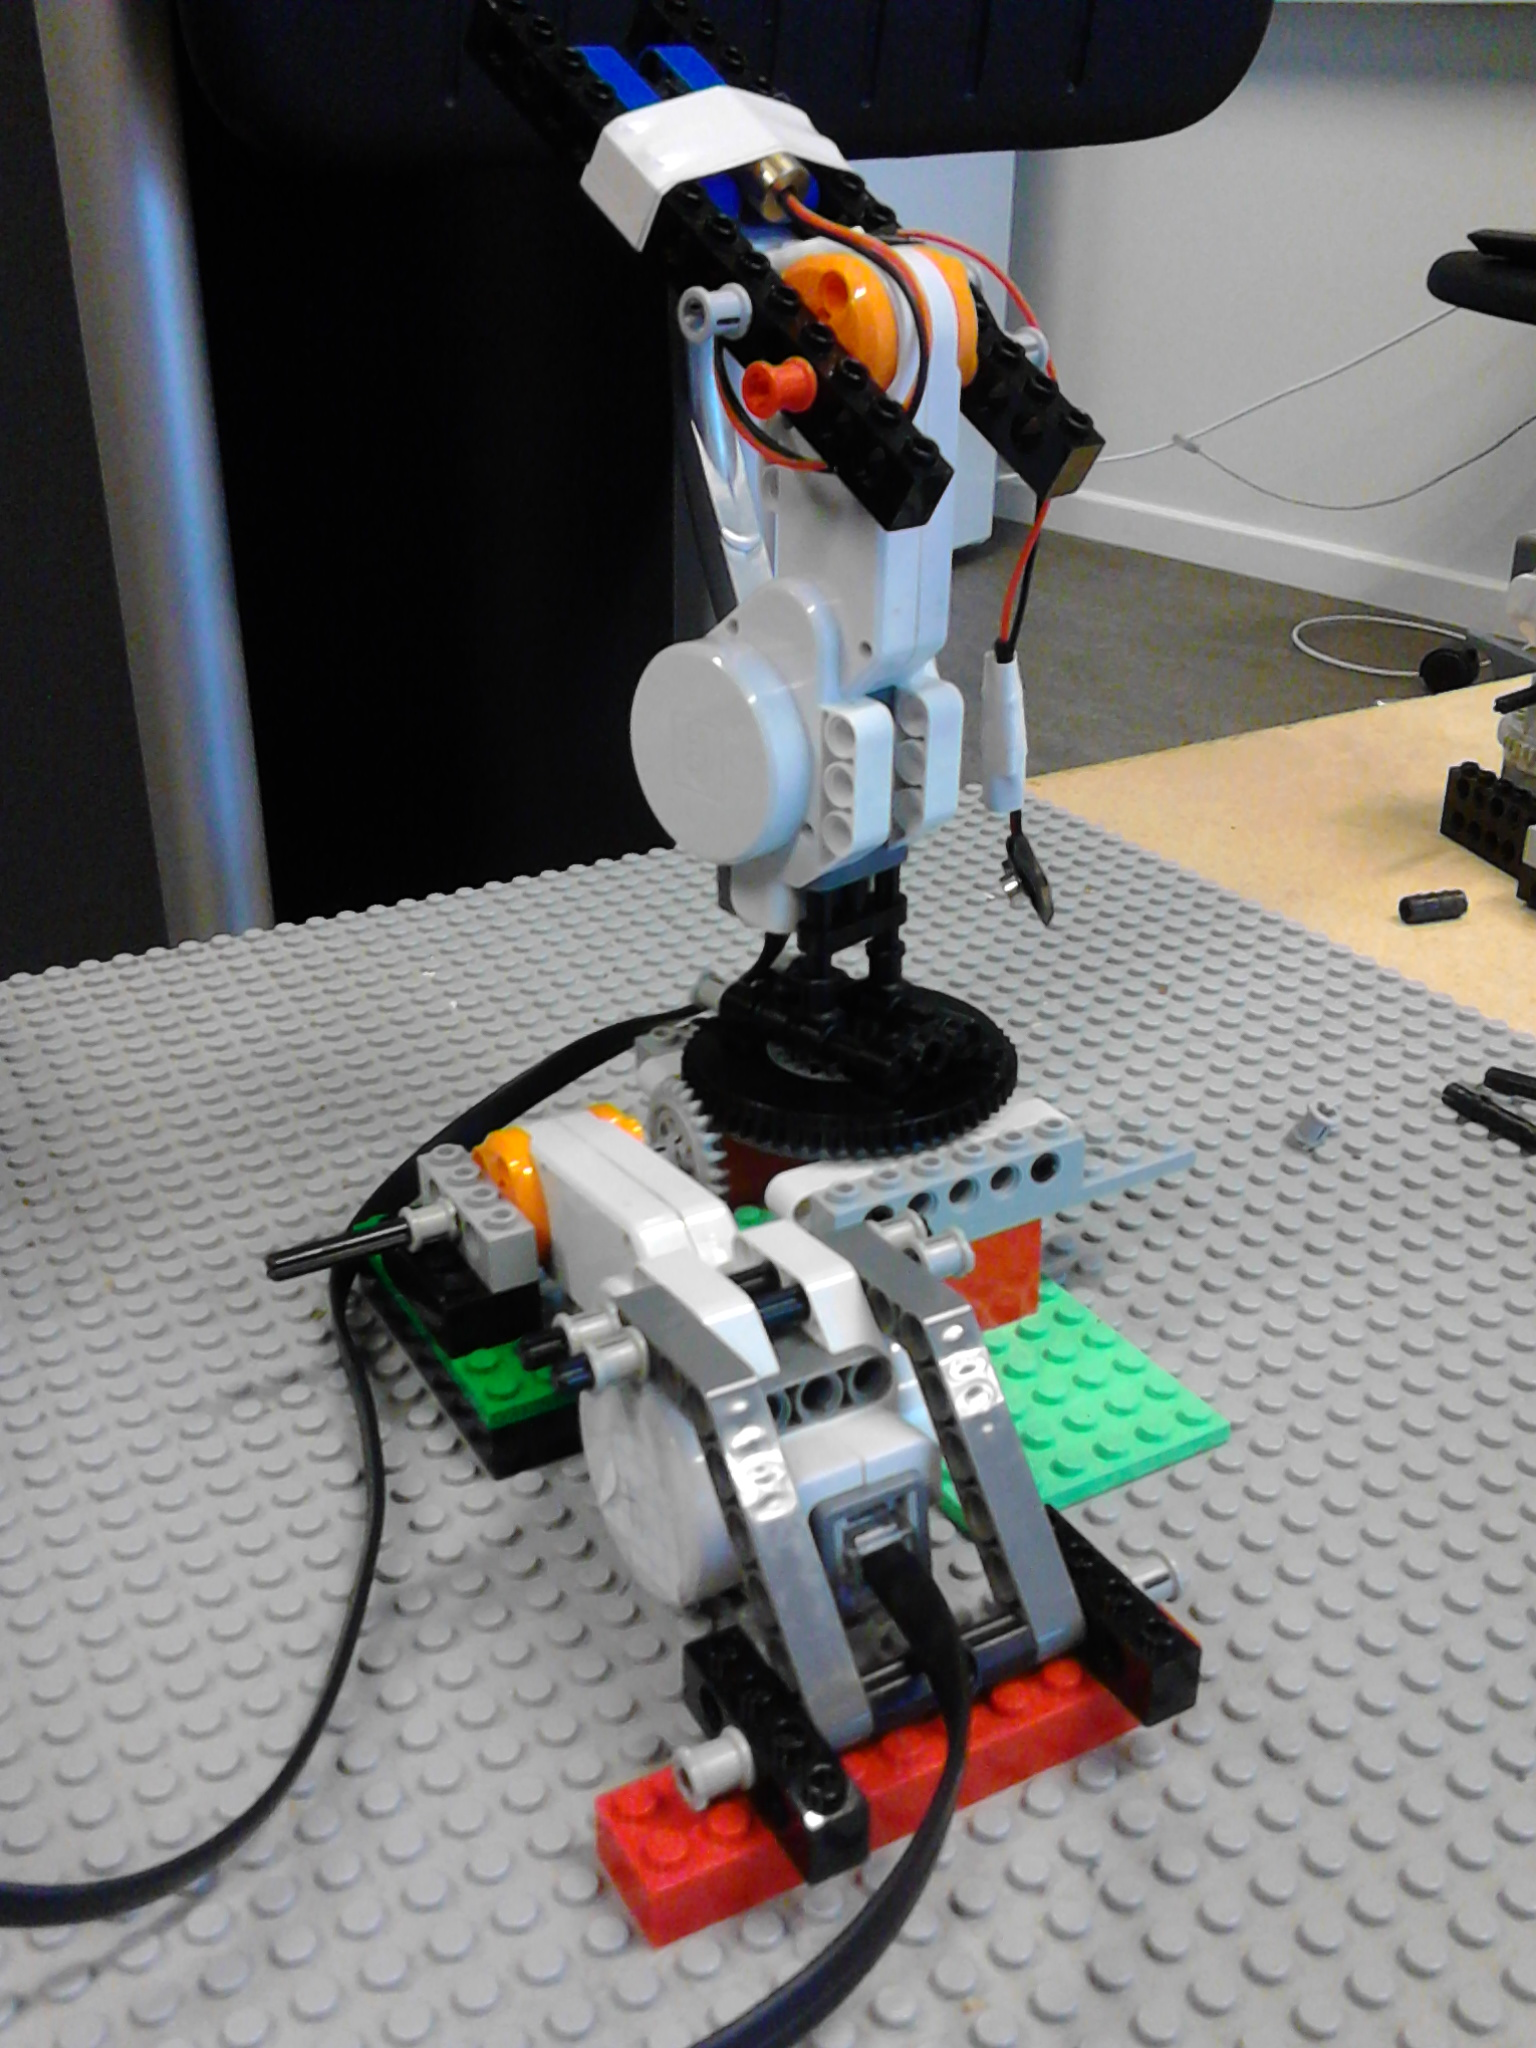
\includegraphics[width=0.50\textwidth]{graphics/rig/rig_standing_entire.jpg}
    \caption{Second setup}
    \label{fig:rig_standing}
\end{figure}

\begin{figure}[H]
    \begin{minipage}{0.5\textwidth}
	\centering
	    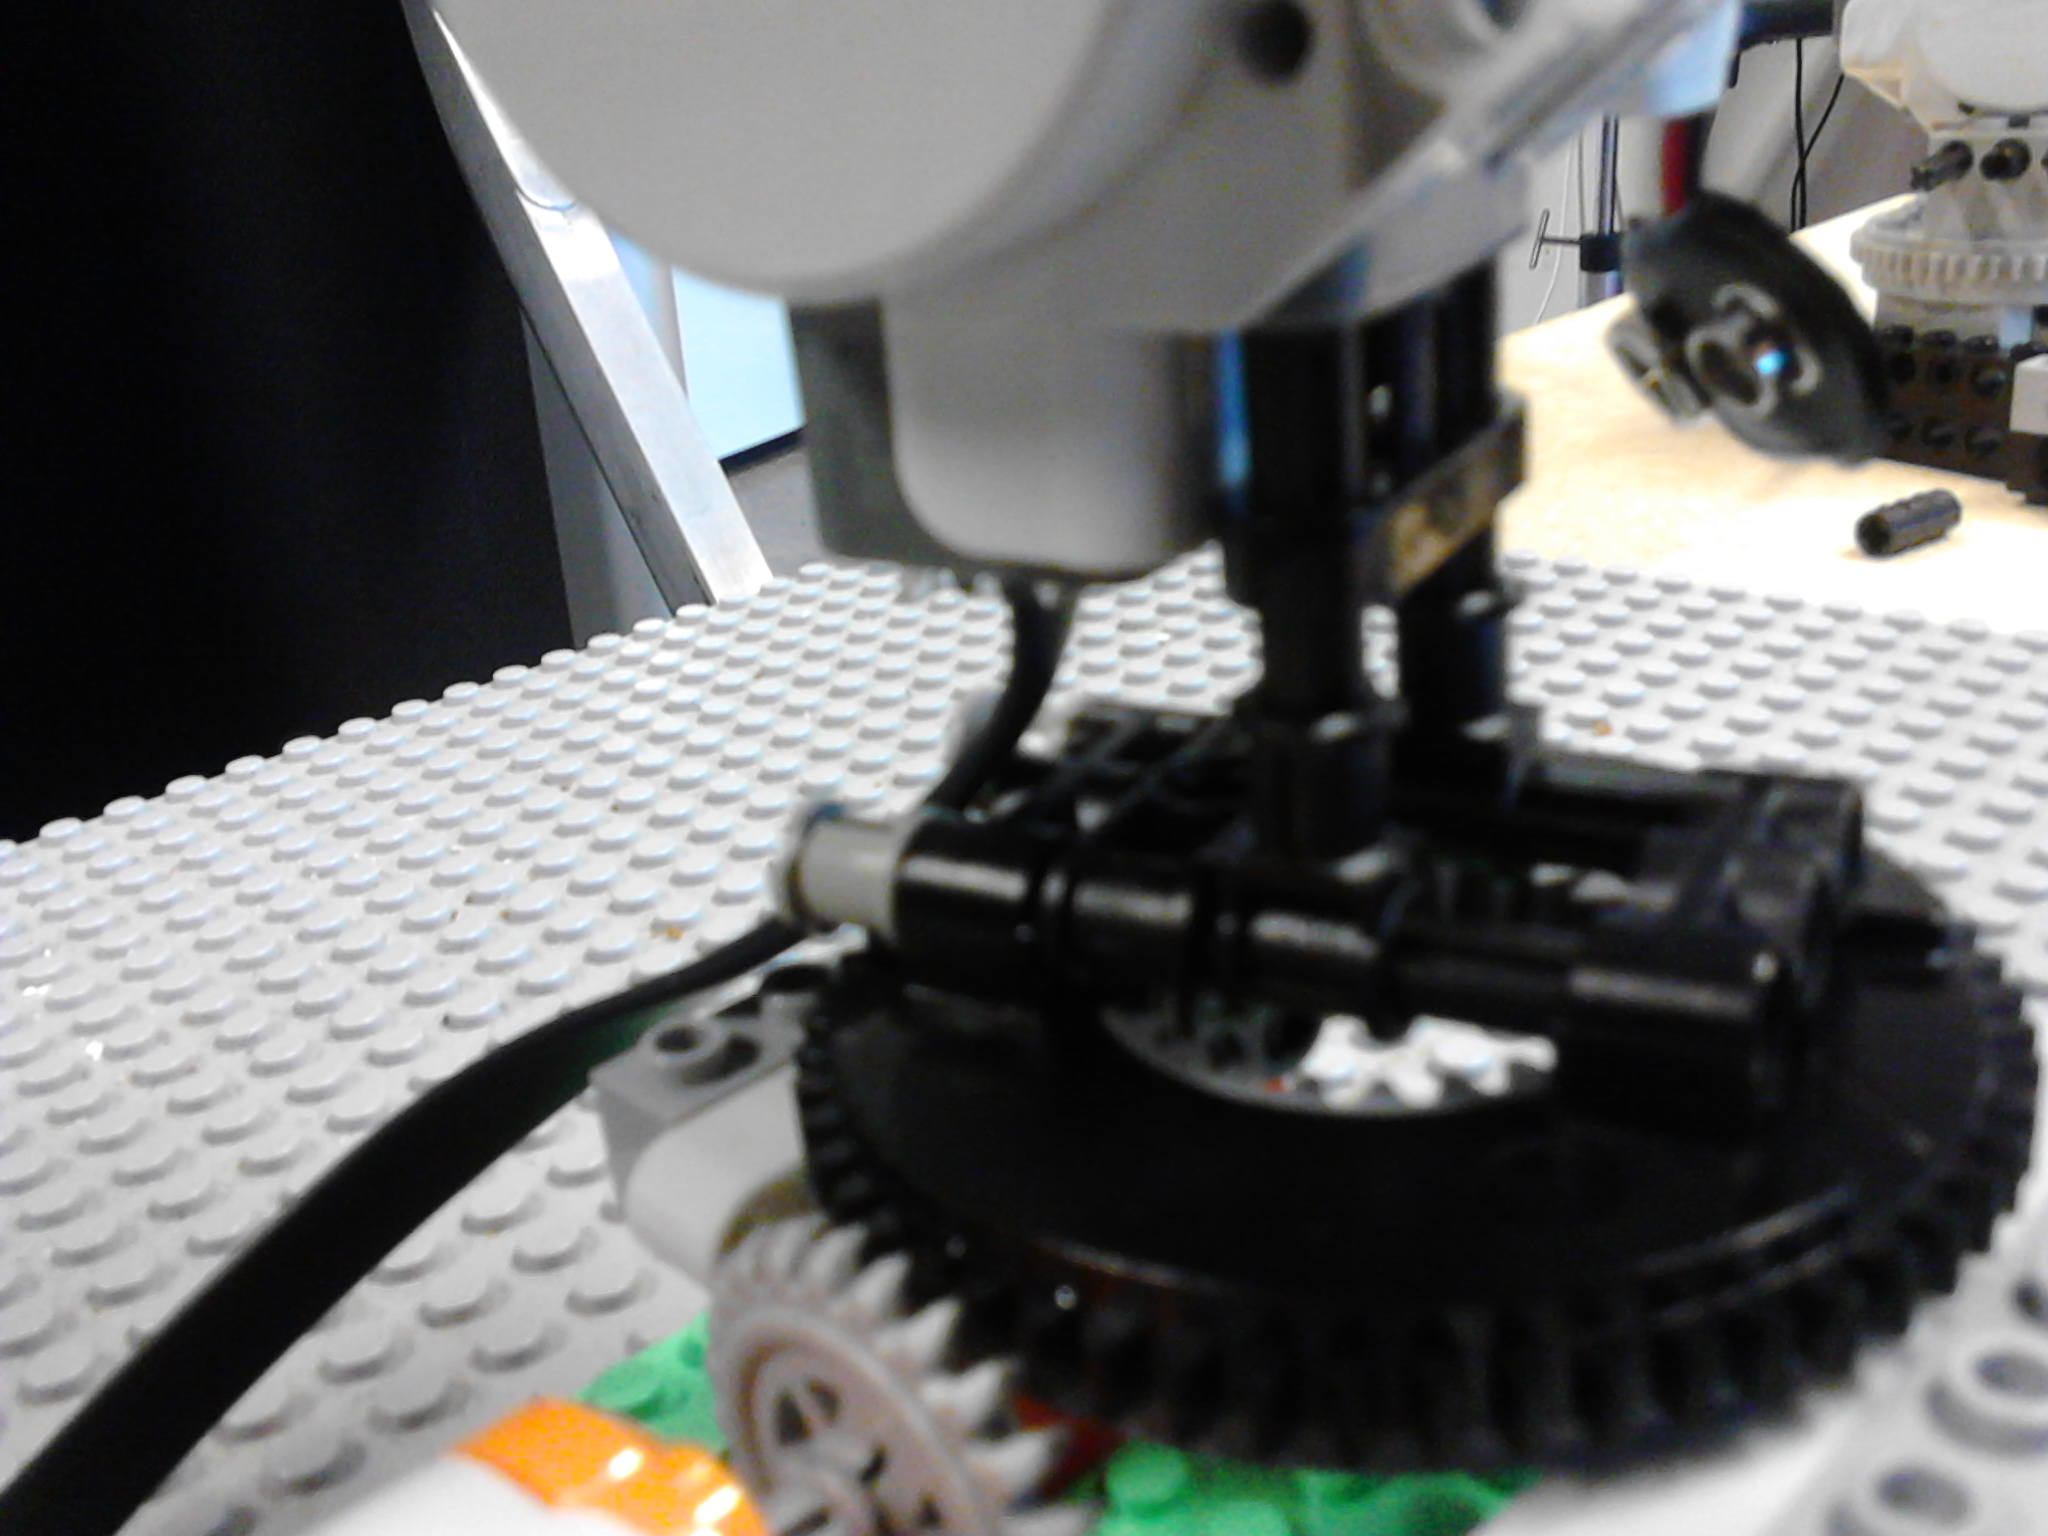
\includegraphics[width=0.80\textwidth]{graphics/rig/rig_standing_unstable.jpg}
	    \caption{Close-up of unstable setup}
	    \label{fig:rig_unstable}
    \end{minipage}%
	\begin{minipage}{0.5\textwidth}
		\centering
	    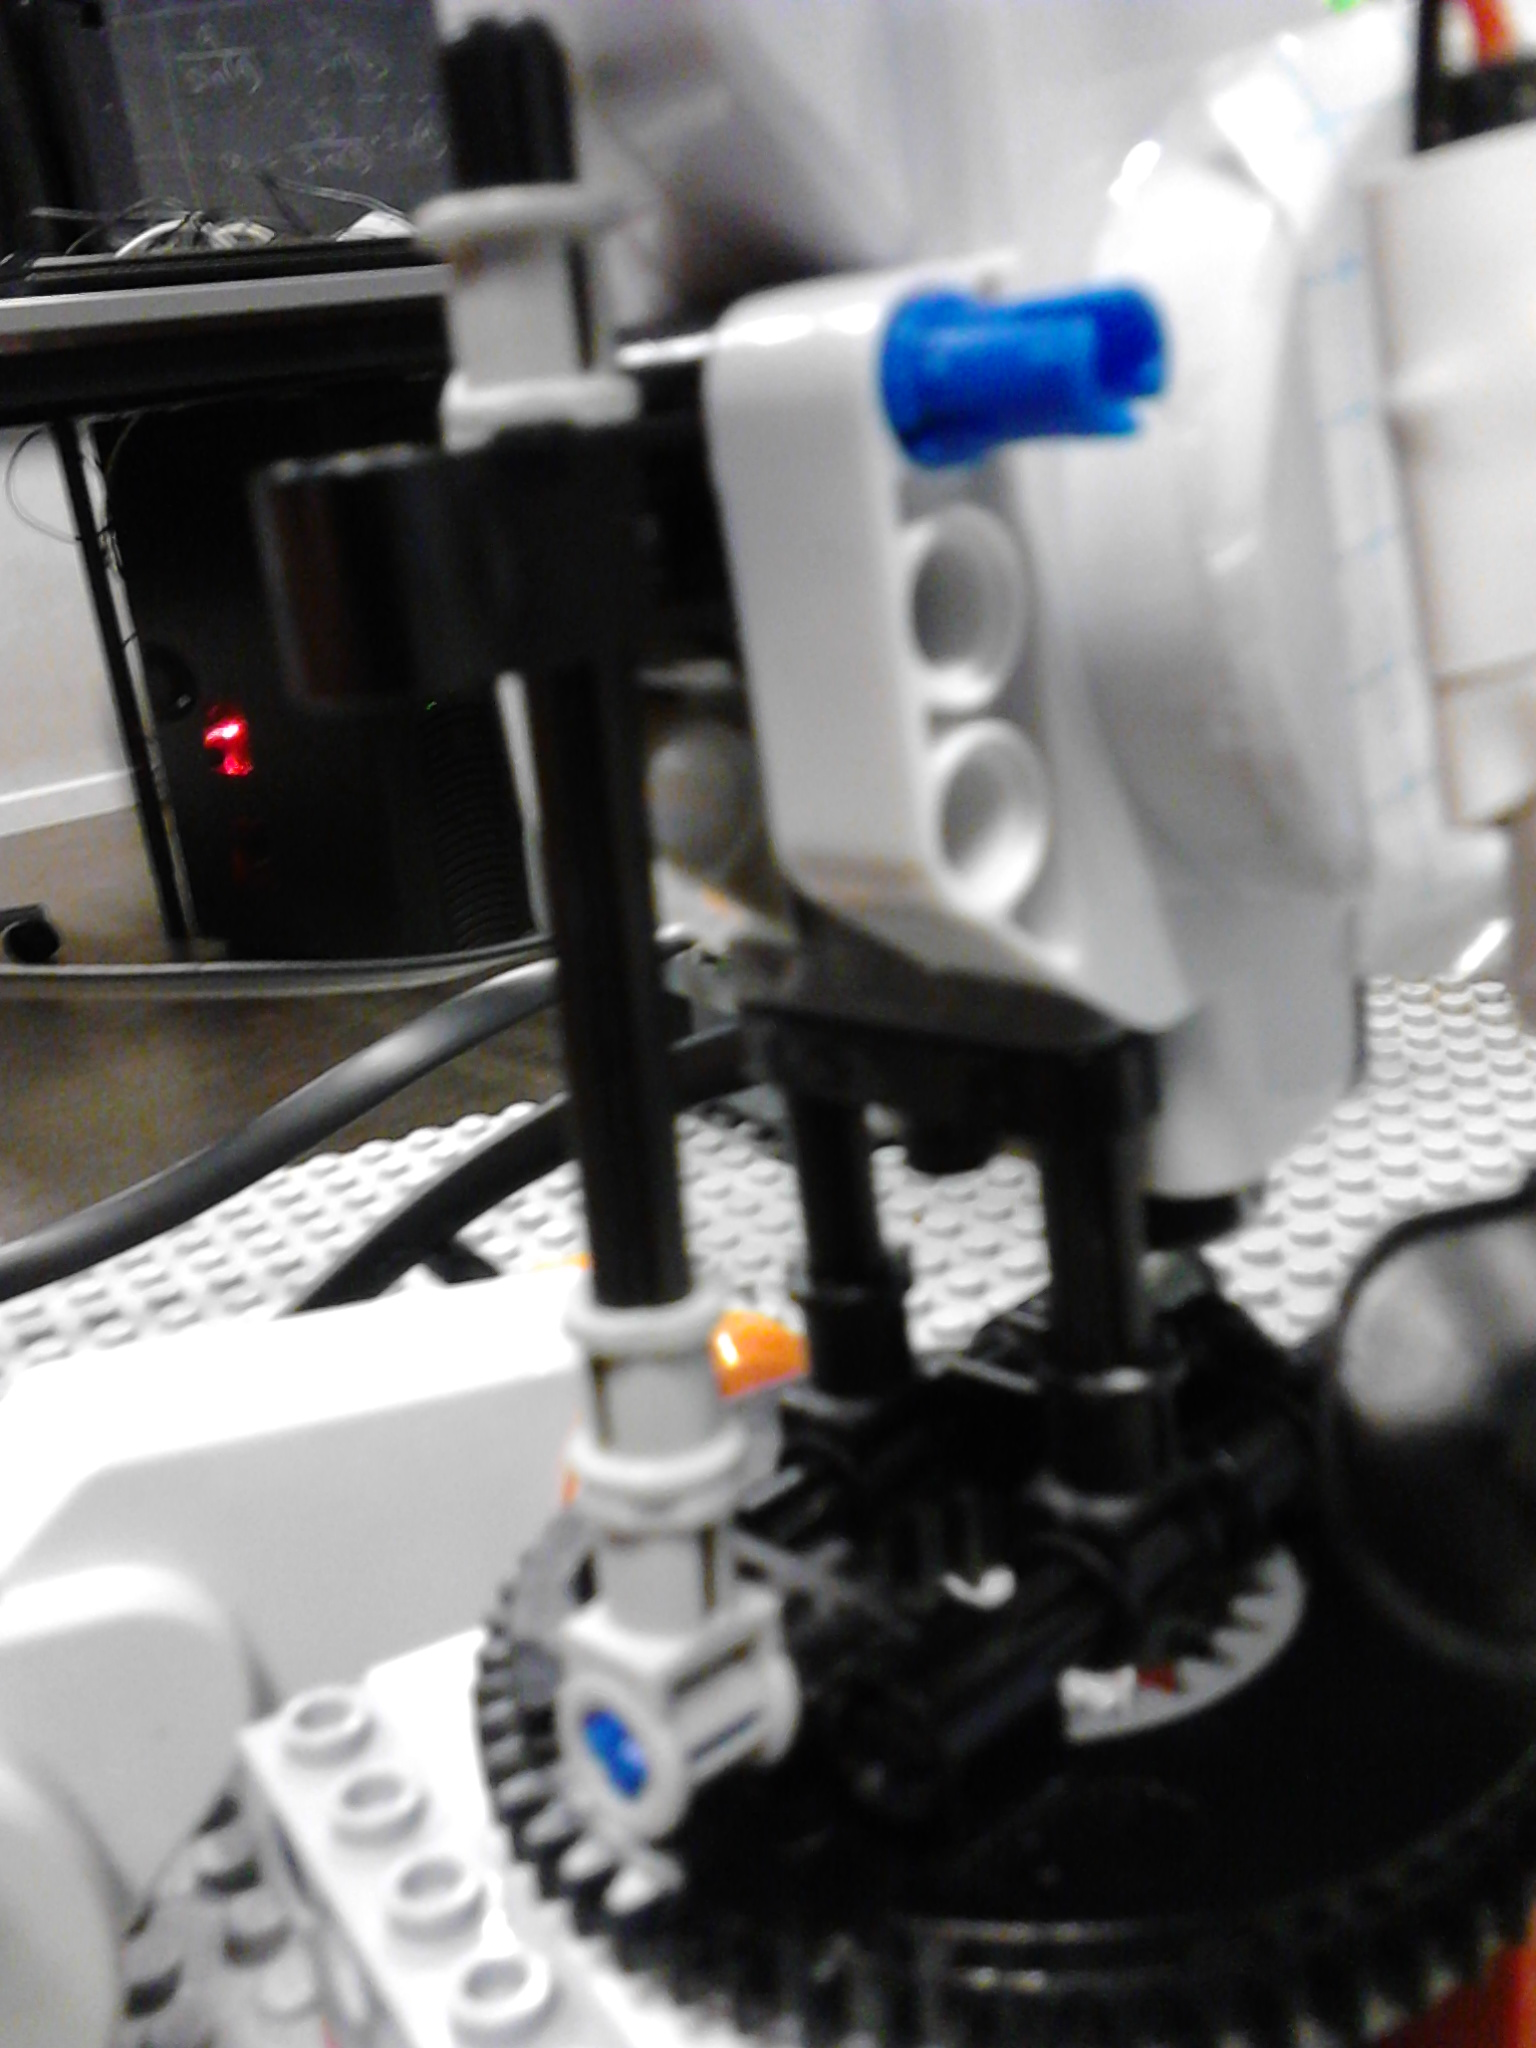
\includegraphics[width=0.80\textwidth]{graphics/rig/rig_standing_stable.jpg}
	    \caption{Close-up of stable setup}
	    \label{fig:rig_stable}
	\end{minipage}
\end{figure}

\section{Final Setup}
The elected setup is the first setup mainly because of its stability. Both setups have the same rotational freedom, therefore it is not taken into consideration. Considering the base points, the vertical base point will be the same, but looking at the horizontal the unstable version of the second setup has great benefits for calculating the base point. However, the instability is to much of a disadvantage. This could be solved for the setup by stabilising it, but that leaves it with the same disadvantages regarding base point, as the first setup. So in the end the benefits and disadvantages will mostly be the same for both setups, other than the first and elected setup being a more stable.